% Options for packages loaded elsewhere
\PassOptionsToPackage{unicode}{hyperref}
\PassOptionsToPackage{hyphens}{url}
%
\documentclass[
]{book}
\usepackage{amsmath,amssymb}
\usepackage{iftex}
\ifPDFTeX
  \usepackage[T1]{fontenc}
  \usepackage[utf8]{inputenc}
  \usepackage{textcomp} % provide euro and other symbols
\else % if luatex or xetex
  \usepackage{unicode-math} % this also loads fontspec
  \defaultfontfeatures{Scale=MatchLowercase}
  \defaultfontfeatures[\rmfamily]{Ligatures=TeX,Scale=1}
\fi
\usepackage{lmodern}
\ifPDFTeX\else
  % xetex/luatex font selection
\fi
% Use upquote if available, for straight quotes in verbatim environments
\IfFileExists{upquote.sty}{\usepackage{upquote}}{}
\IfFileExists{microtype.sty}{% use microtype if available
  \usepackage[]{microtype}
  \UseMicrotypeSet[protrusion]{basicmath} % disable protrusion for tt fonts
}{}
\makeatletter
\@ifundefined{KOMAClassName}{% if non-KOMA class
  \IfFileExists{parskip.sty}{%
    \usepackage{parskip}
  }{% else
    \setlength{\parindent}{0pt}
    \setlength{\parskip}{6pt plus 2pt minus 1pt}}
}{% if KOMA class
  \KOMAoptions{parskip=half}}
\makeatother
\usepackage{xcolor}
\usepackage{longtable,booktabs,array}
\usepackage{calc} % for calculating minipage widths
% Correct order of tables after \paragraph or \subparagraph
\usepackage{etoolbox}
\makeatletter
\patchcmd\longtable{\par}{\if@noskipsec\mbox{}\fi\par}{}{}
\makeatother
% Allow footnotes in longtable head/foot
\IfFileExists{footnotehyper.sty}{\usepackage{footnotehyper}}{\usepackage{footnote}}
\makesavenoteenv{longtable}
\usepackage{graphicx}
\makeatletter
\newsavebox\pandoc@box
\newcommand*\pandocbounded[1]{% scales image to fit in text height/width
  \sbox\pandoc@box{#1}%
  \Gscale@div\@tempa{\textheight}{\dimexpr\ht\pandoc@box+\dp\pandoc@box\relax}%
  \Gscale@div\@tempb{\linewidth}{\wd\pandoc@box}%
  \ifdim\@tempb\p@<\@tempa\p@\let\@tempa\@tempb\fi% select the smaller of both
  \ifdim\@tempa\p@<\p@\scalebox{\@tempa}{\usebox\pandoc@box}%
  \else\usebox{\pandoc@box}%
  \fi%
}
% Set default figure placement to htbp
\def\fps@figure{htbp}
\makeatother
\setlength{\emergencystretch}{3em} % prevent overfull lines
\providecommand{\tightlist}{%
  \setlength{\itemsep}{0pt}\setlength{\parskip}{0pt}}
\setcounter{secnumdepth}{5}
\usepackage{booktabs}
\usepackage[]{natbib}
\bibliographystyle{plainnat}
\usepackage{bookmark}
\IfFileExists{xurl.sty}{\usepackage{xurl}}{} % add URL line breaks if available
\urlstyle{same}
\hypersetup{
  pdftitle={Análisis Series de Tiempo: Precio del Oro},
  pdfauthor={Nicolás Méndez Gutiérrez - Christian Martinez},
  hidelinks,
  pdfcreator={LaTeX via pandoc}}

\title{Análisis Series de Tiempo: Precio del Oro}
\author{Nicolás Méndez Gutiérrez - Christian Martinez}
\date{2025-06-16}

\begin{document}
\maketitle

{
\setcounter{tocdepth}{1}
\tableofcontents
}
\chapter{Descripción del dataset}\label{descripciuxf3n-del-dataset}

Este conjunto de datos contiene registros históricos del precio del oro desde el 31 de diciembre de 2013 hasta el 5 de noviembre de 2024, extraídos del mercado MCX. Se trata de un dataset útil para el análisis de series temporales y la predicción de tendencias del precio del oro.

\section{Estructura de los datos}\label{estructura-de-los-datos}

El dataset incluye 2806 entradas y múltiples columnas con información clave:

\begin{itemize}
\tightlist
\item
  Date: Fecha de transacción.
\item
  Open: Precio de apertura del mercado
\item
  High: Precio más alto alcanzado en el día
\item
  Low: Precio más bajo alcanzado en el día
\item
  Price: Precio de cierre del día
\item
  Volume: Cantidad de transacciones realizadas
\item
  Chg\%: Variación porcentual del precio respecto al día anterior.
\end{itemize}

\chapter{Objetivo}\label{objetivo}

Con este dataset se busca analizar el comportamiento histórico de los precios del oro con el objetivo de identificar tendencias significativas a lo largo del tiempo. Además, permite aplicar modelos estadísticos y de aprendizaje automático para predecir movimientos futuros del mercado, proporcionando herramientas útiles para comprender las dinámicas de este activo financiero y apoyar la toma de decisiones en contextos económicos y de inversión.

\chapter{Justificación}\label{justificaciuxf3n}

El dataset de precios diarios del oro es altamente adecuado para la aplicación de técnicas de análisis de series de tiempo debido a las siguientes características:

\begin{enumerate}
\def\labelenumi{\arabic{enumi}.}
\tightlist
\item
  Datos de tiempo ordenados
\end{enumerate}

\begin{itemize}
\tightlist
\item
  La variable Date proporciona una secuencia cronológica continua sin valores faltantes, lo que facilita la modelación de tendencias y patrones temporales.
\item
  La periodicidad diaria permite estudiar el comportamiento del mercado con alta resolución temporal.
\end{itemize}

\begin{enumerate}
\def\labelenumi{\arabic{enumi}.}
\setcounter{enumi}{1}
\tightlist
\item
  Evolución de variable dependiente
\end{enumerate}

\begin{itemize}
\tightlist
\item
  La columna Price representa el precio de cierre, una métrica clave para analizar la evolución del valor del oro a lo largo del tiempo.
\item
  Al ser una serie numérica con cambios graduales y picos específicos, es ideal para aplicar modelos predictivos como ARIMA, modelos de suavizamiento exponencial y redes neuronales recurrentes.
\end{itemize}

\begin{enumerate}
\def\labelenumi{\arabic{enumi}.}
\setcounter{enumi}{2}
\tightlist
\item
  Factores Exógenos y Multivariabilidad
\end{enumerate}

\begin{itemize}
\tightlist
\item
  Las variables Open, High, Low y Volume permiten estudiar la influencia de distintos factores sobre la variación del precio, enriqueciendo el análisis.
\item
  La columna Chg\% proporciona información sobre volatilidad y puede usarse para identificar momentos de alta inestabilidad en el mercado.
\end{itemize}

\begin{enumerate}
\def\labelenumi{\arabic{enumi}.}
\setcounter{enumi}{3}
\tightlist
\item
  Aplicabilidad Real y Relevancia Económica
\end{enumerate}

\begin{itemize}
\tightlist
\item
  El oro es un activo financiero de gran importancia en la economía global, por lo que analizar sus precios a lo largo del tiempo tiene aplicaciones prácticas en predicción de tendencias, evaluación de riesgos y toma de decisiones de inversión.
\item
  Permite la identificación de patrones estacionales, ciclos de mercado y efectos de eventos económicos en la fluctuación del precio.
\end{itemize}

\begin{enumerate}
\def\labelenumi{\arabic{enumi}.}
\setcounter{enumi}{4}
\tightlist
\item
  Calidad de los datos
\end{enumerate}

\begin{itemize}
\tightlist
\item
  Con 2806 registros sin valores faltantes, el dataset proporciona información confiable para entrenar modelos sin la necesidad de una limpieza exhaustiva.
\item
  La estabilidad en la estructura del dataset facilita la aplicación de metodologías estadísticas y de machine learning.
\end{itemize}

En conclusión este dataset es ideal para estudios de series de tiempo, ya que permite aplicar modelos predictivos, evaluar la influencia de factores exógenos y analizar tendencias económicas con datos sólidos y completos.

\chapter{Análisis Exploratorio de Datos}\label{anuxe1lisis-exploratorio-de-datos}

Se importa el dataset cuyos primeros registros se muestran a continuación.

\begin{verbatim}
# A tibble: 6 x 7
  Date       Price  Open  High   Low Volume `Chg%`
  <date>     <dbl> <dbl> <dbl> <dbl>  <dbl>  <dbl>
1 2024-11-06 77030 78300 78570 77030      0  -1.86
2 2024-11-05 78490 78224 78670 78160      0   0.11
3 2024-11-04 78401 78498 78642 78237      0  -0.54
4 2024-11-01 78829 78650 78887 78550      0   0.64
5 2024-10-31 78326 79264 79999 77803     90  -1.17
6 2024-10-30 79257 79119 79375 78888    130   0.5 
\end{verbatim}

A continuación se presenta un resumen de medidas descriptivas.

\begin{table}

\caption{\label{tab:2}Data summary}
\centering
\begin{tabular}[t]{l|l}
\hline
Name & datos\\
\hline
Number of rows & 2806\\
\hline
Number of columns & 7\\
\hline
\_\_\_\_\_\_\_\_\_\_\_\_\_\_\_\_\_\_\_\_\_\_\_ & \\
\hline
Column type frequency: & \\
\hline
Date & 1\\
\hline
numeric & 6\\
\hline
\_\_\_\_\_\_\_\_\_\_\_\_\_\_\_\_\_\_\_\_\_\_\_\_ & \\
\hline
Group variables & None\\
\hline
\end{tabular}
\end{table}

\textbf{Variable type: Date}

\begin{tabular}{l|r|r|l|l|l|r}
\hline
skim\_variable & n\_missing & complete\_rate & min & max & median & n\_unique\\
\hline
Date & 0 & 1 & 2014-01-01 & 2024-11-06 & 2019-05-27 & 2806\\
\hline
\end{tabular}

\textbf{Variable type: numeric}

\begin{tabular}{l|r|r|r|r|r|r|r|r|r|l}
\hline
skim\_variable & n\_missing & complete\_rate & mean & sd & p0 & p25 & p50 & p75 & p100 & hist\\
\hline
Price & 0 & 1 & 40699.89 & 13828.62 & 24545.00 & 29128.00 & 32980.00 & 50613.50 & 79257.0 & ▇▂▃▂▁\\
\hline
Open & 0 & 1 & 40700.22 & 13826.94 & 24583.00 & 29103.75 & 33000.00 & 50646.75 & 79264.0 & ▇▂▃▂▁\\
\hline
High & 0 & 1 & 40917.78 & 13900.47 & 24635.00 & 29261.25 & 33220.50 & 50911.25 & 79999.0 & ▇▂▃▂▁\\
\hline
Low & 0 & 1 & 40482.31 & 13756.09 & 24470.00 & 28974.00 & 32890.00 & 50337.50 & 78888.0 & ▇▂▃▂▁\\
\hline
Volume & 0 & 1 & 12529.58 & 10649.99 & 0.00 & 6282.50 & 10770.00 & 16397.50 & 106920.0 & ▇▁▁▁▁\\
\hline
Chg\% & 0 & 1 & 0.04 & 0.83 & -5.98 & -0.38 & 0.04 & 0.45 & 5.3 & ▁▁▇▁▁\\
\hline
\end{tabular}

Se explora la existencia de datos faltantes.

\begin{verbatim}
  Date  Price   Open   High    Low Volume   Chg% 
     0      0      0      0      0      0      0 
\end{verbatim}

Se realizan gráficos para observar tendencias a lo largo del tiempo de:

\begin{itemize}
\item
  El precio
  \pandocbounded{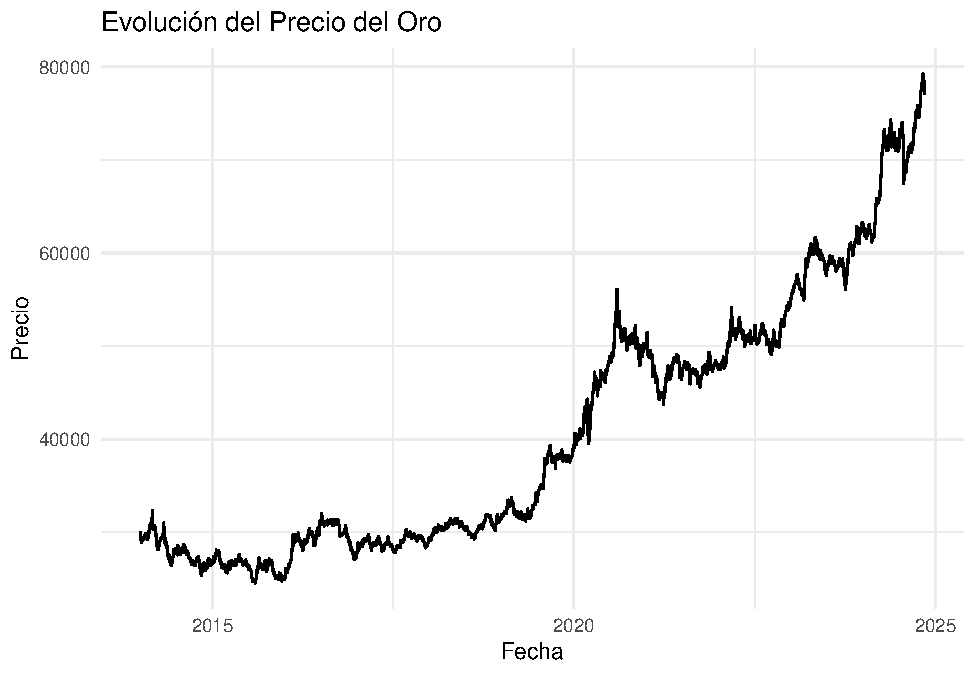
\includegraphics[keepaspectratio]{_main_files/figure-latex/4-1.pdf}}
\item
  Cambios porcentuales
  \pandocbounded{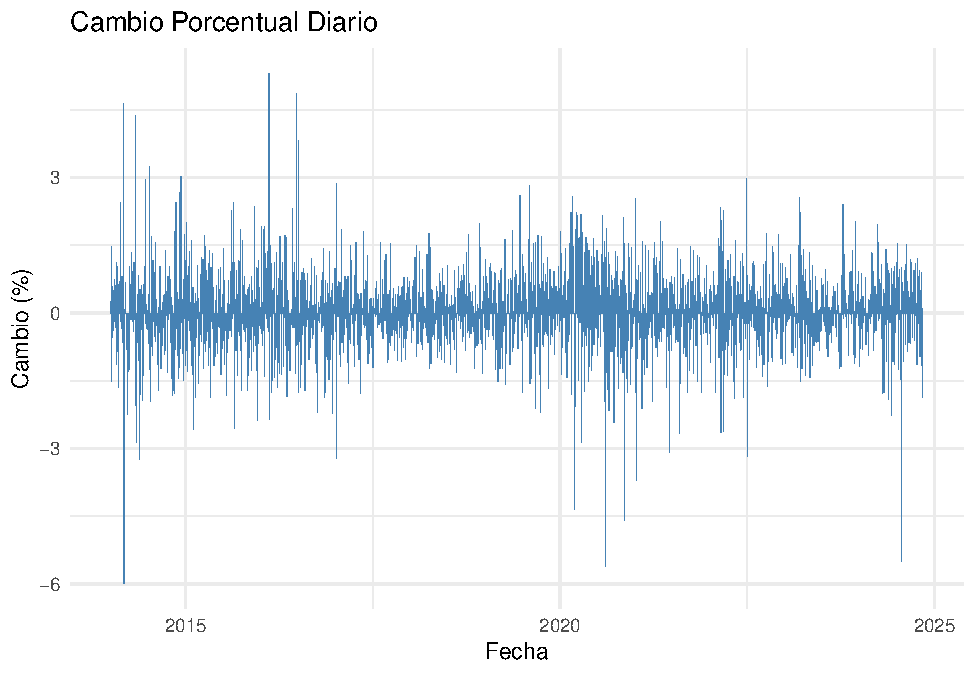
\includegraphics[keepaspectratio]{_main_files/figure-latex/5-1.pdf}}
\item
  Comparación del valor máximo vs mínimos del día
  \pandocbounded{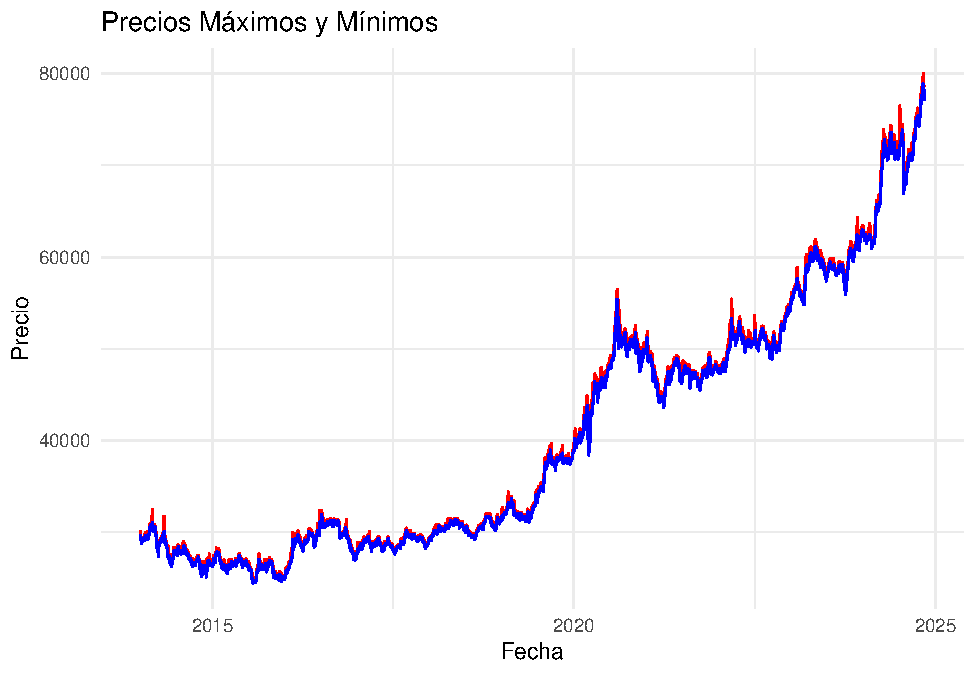
\includegraphics[keepaspectratio]{_main_files/figure-latex/6-1.pdf}}
\end{itemize}

\section{Análisis de promedio movil, rezagos y estacionalidad}\label{anuxe1lisis-de-promedio-movil-rezagos-y-estacionalidad}

\subsection{Promedio móvil}\label{promedio-muxf3vil}

Se agrega un promedio móvil de 7 días, es decir, de manera semanal ya que muchos mercados (como el oro, acciones, productos básicos) tienden a mostrar variaciones semanales
(por factores como fin de semana, cierres de mercado, ciclos de noticias, etc.)

\pandocbounded{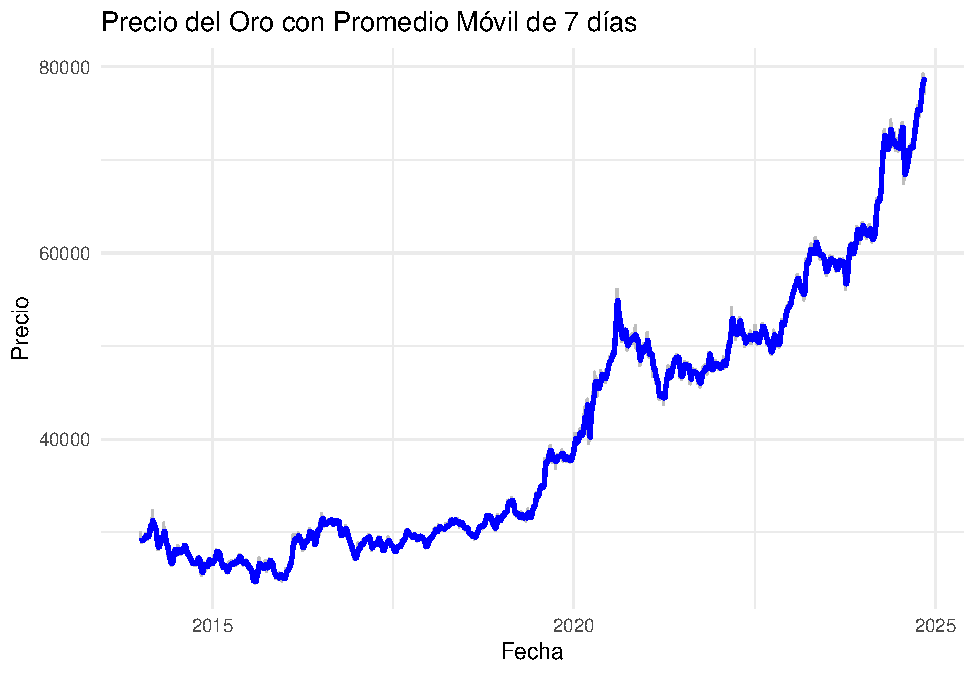
\includegraphics[keepaspectratio]{_main_files/figure-latex/8-1.pdf}}

Se hacen las siguientes observaciones:

\begin{itemize}
\tightlist
\item
  La serie muestra una tendencia creciente de largo plazo, especialmente desde 2019 en adelante.
\item
  2013 - 2018: El precio del oro estuvo relativamente estable o ligeramente a la baja, con pequeñas fluctuaciones.
\item
  2019 - 2020: Se observa un fuerte crecimiento, con un aumento pronunciado en el precio.
\item
  2020 - 2021: Hay una corrección o caída parcial, después de un máximo.
\item
  2021 - 2025: Retoma una tendencia alcista constante con algunos ciclos de subida y bajada.
\item
  Se identifican momentos donde la curva cambia de pendiente (subidas abruptas o correcciones), que pueden estar asociadas a eventos macroeconómicos.
\end{itemize}

\subsection{Rezagos (lags)}\label{rezagos-lags}

\pandocbounded{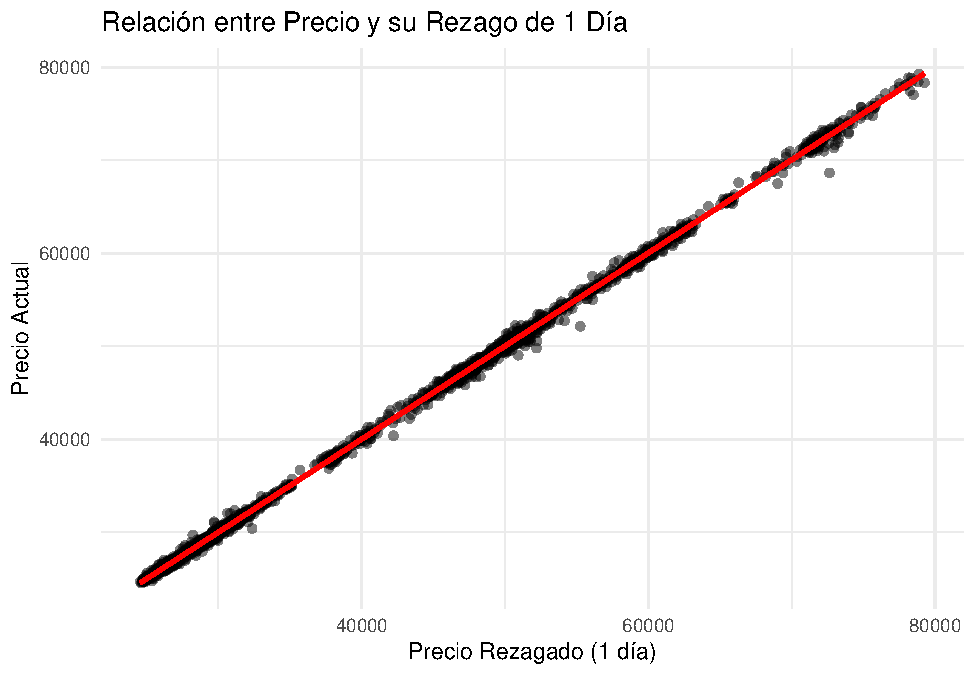
\includegraphics[keepaspectratio]{_main_files/figure-latex/9-1.pdf}}

Se realizan las siguientes observaciones:

\begin{itemize}
\tightlist
\item
  El precio del oro no cambia drásticamente de un día para otro; más bien tiende a seguir la misma trayectoria.
\item
  Hay baja volatilidad diaria relativa (aunque a largo plazo se observaron tendencias importantes).
\end{itemize}

\subsection{Estacionalidad}\label{estacionalidad}

\pandocbounded{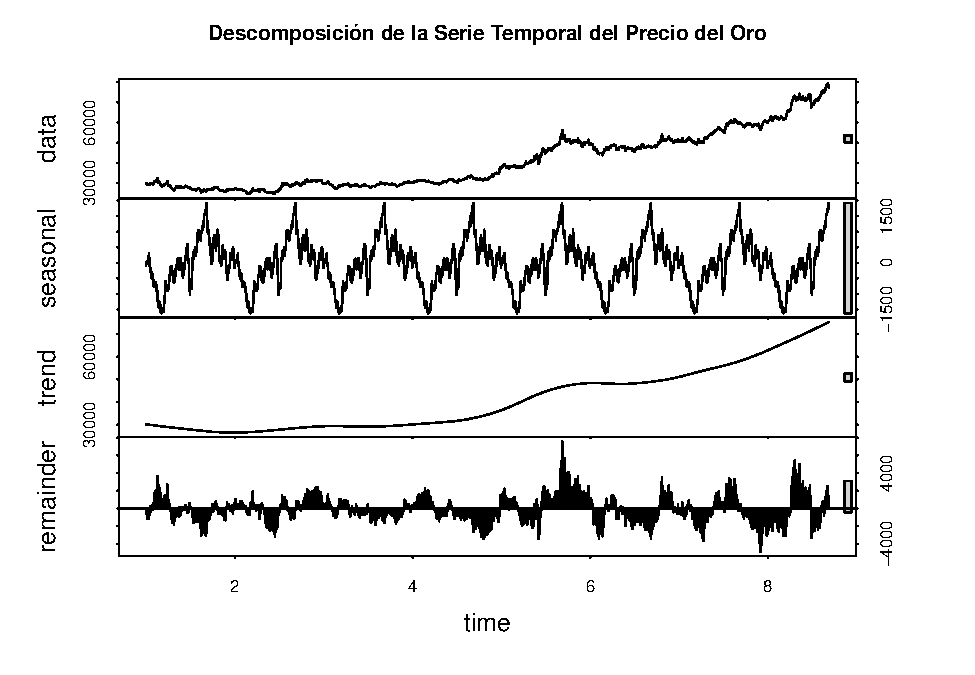
\includegraphics[keepaspectratio]{_main_files/figure-latex/10-1.pdf}}

\begin{itemize}
\tightlist
\item
  En la primera porción de la gráfica, se observa el comportamiento de la variable precio a lo largo del tiempo.
\item
  La segunda porción, Seasonal, muestra cómo varía sistemáticamente a lo largo del año.
\item
  La tercera porción, muestra la Tendencia a largo plazo.
\item
  Finalmente, se observa en la porción de Remainder el ruido no se explicado por la estacionalidad.
\end{itemize}

De la gráfica, se realizan las siguientes observaciones:

\begin{itemize}
\tightlist
\item
  Se aprecia claramente la tendencia creciente fuerte, especialmente desde el año 2020 en adelante.
\item
  El componente estacional muestra ciclos repetitivos con una frecuencia regular de picos y valles aproximadamente cada año. La amplitud del patrón estacional es pequeña en comparación al nivel del precio.
\end{itemize}

Se verifica la estacionalidad.

\begin{verbatim}

    Augmented Dickey-Fuller Test

data:  serie_ts
Dickey-Fuller = -1.2393, Lag order = 14, p-value = 0.9002
alternative hypothesis: stationary
\end{verbatim}

\begin{itemize}
\tightlist
\item
  El ADF test evalúa la hipótesis nula de que una serie no es estacionaria (tiene raíz unitaria), frente a la hipótesis alternativa de que sí es estacionaria.
\item
  Con un p-valor tan alto (0.9002), la evidencia estadística indica que la serie ts\_price:

  \begin{itemize}
  \tightlist
  \item
    No tiene media ni varianza constante en el tiempo.
  \item
    Tiene una tendencia persistente, como ya se vio en la descomposición STL.
  \item
    No es apta para modelado directo con ARIMA u otras técnicas que requieren estacionariedad, a menos que se transforme.
  \end{itemize}
\end{itemize}

\subsection{Diferenciación de primer orden}\label{diferenciaciuxf3n-de-primer-orden}

\pandocbounded{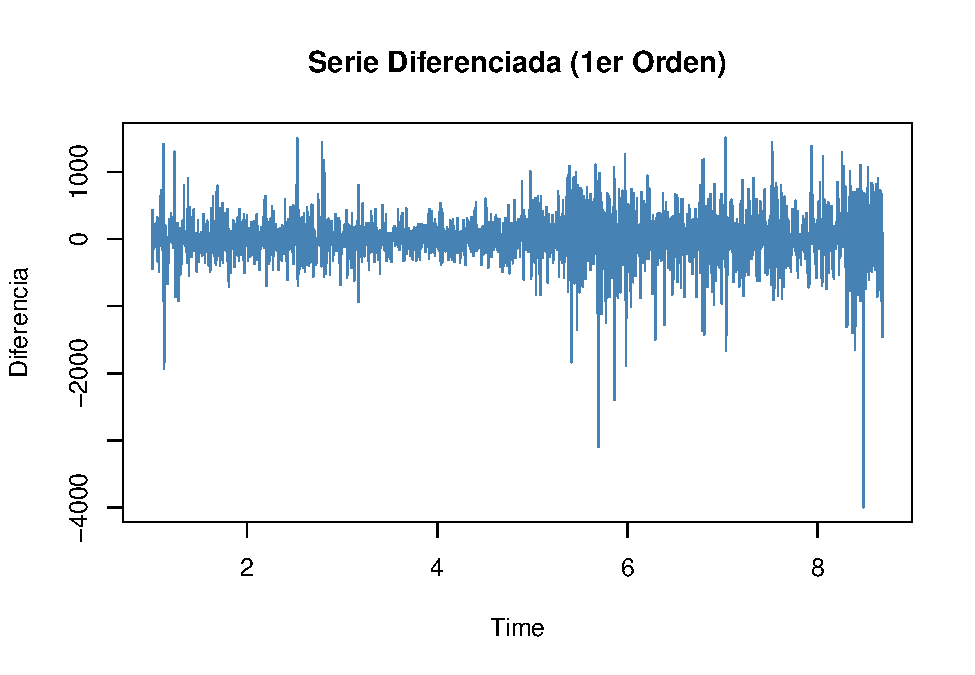
\includegraphics[keepaspectratio]{_main_files/figure-latex/12-1.pdf}}

Prueba ADF tras la diferenciación:

\begin{verbatim}

    Augmented Dickey-Fuller Test

data:  ts_diff1
Dickey-Fuller = -15.197, Lag order = 14, p-value = 0.01
alternative hypothesis: stationary
\end{verbatim}

\begin{itemize}
\tightlist
\item
  p-value = 0.01: Significa que podemos rechazar la hipótesis nula de no estacionariedad.
\item
  El estadístico Dickey-Fuller altamente negativo (-15.197) indica una fuerte evidencia de estacionariedad.
\end{itemize}

\subsection{Transformación logarítmica + diferencia}\label{transformaciuxf3n-logaruxedtmica-diferencia}

\pandocbounded{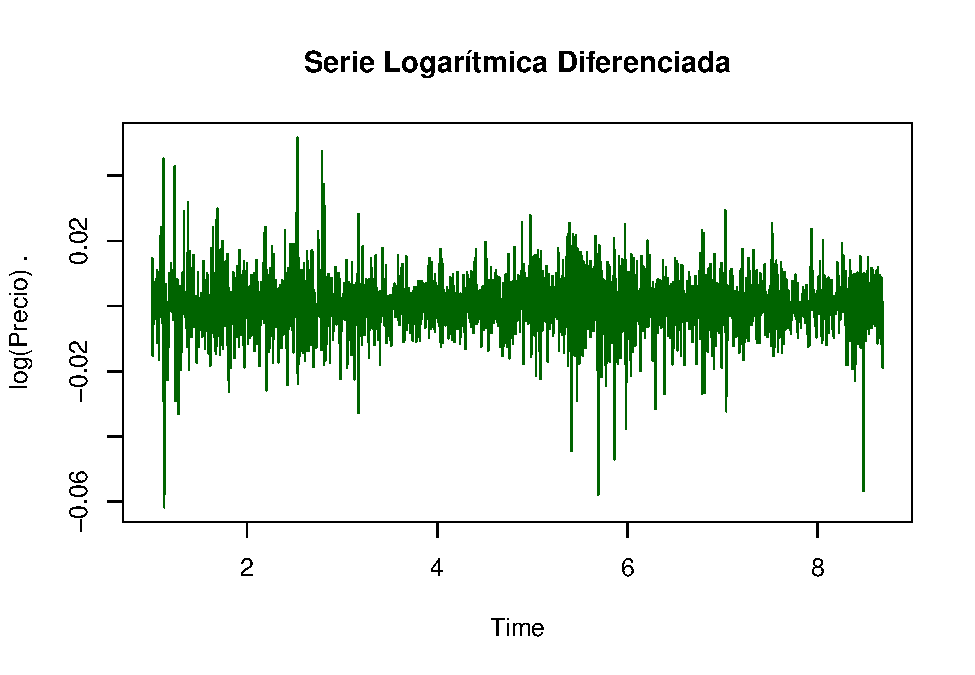
\includegraphics[keepaspectratio]{_main_files/figure-latex/14-1.pdf}}

\begin{itemize}
\tightlist
\item
  La serie resultante oscila en torno a cero, lo cual indica estacionariedad en media.
\item
  No hay una tendencia visible: el promedio es constante.
\item
  La dispersión (volatilidad) se ve bastante estable a lo largo del tiempo → varianza constante, o al menos más homogénea que la serie original.
\item
  Hay algunos picos puntuales que pueden ser eventos de mercado extremos, pero no afectan la estructura general.
\item
  La serie logarítmica diferenciada cumple con los requisitos clave de una serie estacionaria: media constante, varianza relativamente constante y ausencia de tendencia.
\item
  Es altamente recomendable trabajar con esta serie transformada para fines de modelado, predicción o análisis estadístico.
\end{itemize}

ADF para log-diff:

\begin{verbatim}

    Augmented Dickey-Fuller Test

data:  ts_log_diff
Dickey-Fuller = -14.322, Lag order = 14, p-value = 0.01
alternative hypothesis: stationary
\end{verbatim}

\begin{itemize}
\tightlist
\item
  Se aplicó la transformación logarítmica y diferenciación de primer orden a la serie del precio del oro con el objetivo de controlar la tendencia creciente y la variabilidad no constante observadas en la serie original.
\item
  La prueba de Dickey-Fuller aumentada aplicada a la serie transformada (diff(log(Precio))) arrojó un estadístico de -14.322 y un p-valor inferior a 0.01, lo cual permite rechazar la hipótesis nula de no estacionariedad.
\item
  Por tanto, se concluye que la serie logarítmica diferenciada es estacionaria, lo cual justifica su uso en procesos de modelado como ARIMA, SARIMA o técnicas de pronóstico más avanzadas. Esta transformación también normaliza la escala de los cambios, permitiendo interpretar los resultados en términos de retornos porcentuales diarios.
\end{itemize}

\subsection{Visualización comparativa}\label{visualizaciuxf3n-comparativa}

\pandocbounded{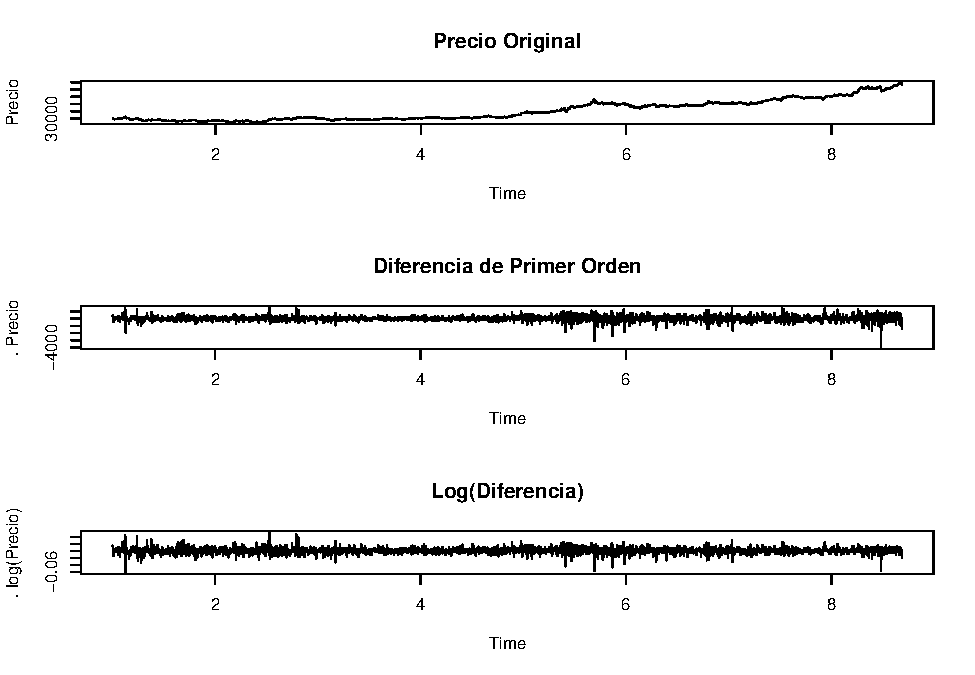
\includegraphics[keepaspectratio]{_main_files/figure-latex/16-1.pdf}}

\begin{itemize}
\tightlist
\item
  La serie original del precio del oro presenta una tendencia creciente y varianza heterogénea, por lo que no cumple los requisitos de estacionariedad
\item
  La diferenciación de primer orden elimina la tendencia, estabilizando la media pero no completamente la varianza.
\item
  Al aplicar una transformación logarítmica seguida de una diferencia, se consigue una serie que oscila alrededor de cero y mantiene varianza aproximadamente constante.
\end{itemize}

\chapter{Pronóstico de Series de Tiempo Holt-Winters}\label{pronuxf3stico-de-series-de-tiempo-holt-winters}

\section{Aplicar el modelo de Holt-Winters}\label{aplicar-el-modelo-de-holt-winters}

Dado que la estacionalidad parece mantenerse relativamente constante en magnitud, un modelo aditivo podría ser la mejor opción.
\pandocbounded{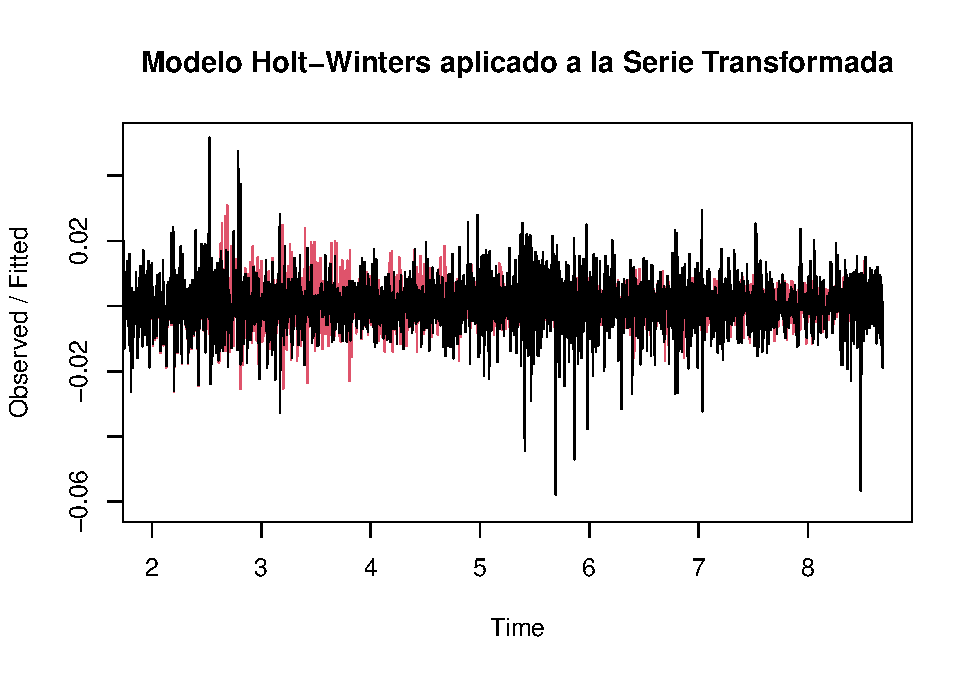
\includegraphics[keepaspectratio]{_main_files/figure-latex/17-1.pdf}}

\section{Evaluar el ajuste del modelo}\label{evaluar-el-ajuste-del-modelo}

\begin{verbatim}
Holt-Winters exponential smoothing with trend and additive seasonal component.

Call:
HoltWinters(x = ts_log_diff, seasonal = "additive")

Smoothing parameters:
 alpha: 0.002485839
 beta : 0.002304457
 gamma: 0.3500246

Coefficients:
              [,1]
a     1.089413e-03
b     2.932241e-07
s1   -6.006596e-03
s2    1.246027e-03
s3   -8.027069e-03
s4   -2.008704e-03
s5    2.991473e-04
s6   -8.319845e-04
s7   -8.802151e-05
s8   -2.843903e-05
s9   -4.982854e-03
s10  -2.517230e-03
s11  -2.391878e-03
s12  -5.668210e-03
s13  -1.517069e-03
s14   4.203068e-03
s15  -5.860747e-03
s16  -4.513237e-03
s17  -6.195080e-03
s18   2.270634e-03
s19  -9.076049e-04
s20   1.097961e-03
s21  -4.155383e-04
s22   1.418486e-03
s23   2.978348e-03
s24   1.081771e-03
s25   2.798766e-03
s26   2.399658e-03
s27   8.182494e-04
s28   4.736225e-03
s29  -3.317307e-03
s30   1.932720e-03
s31   3.491386e-03
s32  -5.864551e-03
s33  -2.540030e-03
s34  -3.128440e-03
s35   1.668221e-04
s36   4.548463e-03
s37  -8.277647e-03
s38   6.471696e-03
s39   3.618264e-03
s40  -5.832373e-03
s41   3.544630e-03
s42   6.176063e-04
s43   3.768946e-03
s44   3.233909e-03
s45  -8.607834e-03
s46   1.886078e-03
s47  -4.186039e-03
s48  -4.515139e-03
s49  -4.135955e-03
s50  -6.368050e-03
s51  -8.977087e-04
s52  -3.290024e-03
s53   1.113716e-03
s54  -3.342337e-03
s55   3.626755e-03
s56  -3.965273e-04
s57  -2.075680e-03
s58  -2.754280e-03
s59  -1.405891e-03
s60   4.118341e-03
s61   4.136166e-03
s62   5.349444e-04
s63  -1.192350e-04
s64   3.438841e-03
s65  -8.287332e-04
s66  -6.952767e-03
s67  -2.787879e-04
s68  -1.830619e-03
s69   1.436565e-03
s70   6.209574e-04
s71  -5.218110e-04
s72   3.209954e-03
s73  -1.704215e-03
s74  -1.688774e-03
s75   2.952404e-04
s76  -3.293497e-03
s77  -4.826419e-03
s78  -2.566117e-03
s79  -4.163923e-03
s80  -5.329070e-03
s81  -2.842959e-03
s82  -6.989766e-03
s83  -1.787856e-03
s84  -2.049335e-03
s85   1.667841e-03
s86   4.879011e-03
s87   4.247008e-03
s88  -3.933419e-04
s89   3.012296e-05
s90  -5.543990e-03
s91   6.826864e-03
s92   8.567619e-05
s93  -2.883496e-04
s94   4.622209e-03
s95   5.927811e-03
s96   1.775474e-03
s97   8.635489e-04
s98  -1.558136e-03
s99  -3.130259e-04
s100 -1.621674e-03
s101  1.923294e-03
s102 -1.312027e-03
s103 -3.636532e-04
s104 -3.493332e-03
s105  3.553864e-03
s106  3.928525e-03
s107  4.448884e-06
s108 -4.001756e-03
s109  4.056982e-04
s110 -6.927393e-03
s111  1.478844e-05
s112 -4.999524e-03
s113 -3.199070e-03
s114  3.233633e-03
s115  6.957504e-04
s116  1.863936e-03
s117 -4.423341e-04
s118  1.509581e-03
s119  2.021815e-03
s120 -1.846520e-03
s121 -8.005496e-04
s122  1.547061e-03
s123  7.182702e-04
s124  3.714035e-03
s125 -4.027189e-03
s126  5.717808e-03
s127  1.090861e-03
s128 -6.418397e-03
s129 -6.786928e-03
s130 -2.867290e-04
s131  6.528340e-05
s132 -6.009571e-03
s133 -6.327125e-03
s134 -2.976976e-04
s135 -4.604251e-03
s136  6.340743e-03
s137 -3.164186e-03
s138 -1.556197e-03
s139 -2.462869e-04
s140  1.099738e-03
s141  1.735485e-03
s142 -5.319717e-04
s143 -3.608170e-03
s144  1.684462e-03
s145 -1.790658e-03
s146 -3.481895e-03
s147 -1.779749e-03
s148  5.323218e-04
s149 -6.065902e-03
s150  1.716859e-03
s151  1.219301e-03
s152 -1.874268e-04
s153  3.829110e-04
s154 -4.783010e-03
s155  1.612731e-05
s156  2.364233e-03
s157 -2.213734e-03
s158 -5.597966e-03
s159 -3.821089e-03
s160 -1.373256e-03
s161 -1.532013e-03
s162 -1.285978e-03
s163 -8.144388e-04
s164 -5.205727e-04
s165 -6.249899e-03
s166 -4.720708e-04
s167 -1.068796e-03
s168  4.517868e-03
s169 -6.817660e-04
s170 -1.010070e-03
s171  1.062472e-03
s172 -1.666314e-03
s173 -1.761655e-03
s174 -4.016522e-03
s175  1.751336e-03
s176 -2.530273e-03
s177 -2.995931e-03
s178 -1.441361e-03
s179 -1.575449e-03
s180  3.343202e-03
s181  4.673575e-04
s182 -2.332107e-03
s183 -5.178601e-04
s184  3.990410e-04
s185 -2.133255e-03
s186 -2.094731e-03
s187 -3.896340e-04
s188  1.691047e-03
s189  3.578948e-03
s190  3.145779e-03
s191  9.474957e-04
s192  1.053631e-02
s193  6.194174e-03
s194  3.225156e-03
s195 -2.621365e-04
s196 -5.642724e-03
s197 -3.521495e-03
s198  1.971002e-03
s199 -1.263471e-03
s200 -4.996198e-03
s201  1.445967e-03
s202 -1.776308e-03
s203 -2.344029e-03
s204  1.617864e-03
s205  1.496596e-03
s206  3.895873e-04
s207  1.367554e-03
s208  6.668821e-04
s209  7.164653e-03
s210  6.009623e-04
s211  4.941777e-03
s212  1.448600e-03
s213  2.806936e-04
s214  3.264814e-03
s215  1.906557e-03
s216  3.418660e-03
s217  1.675327e-03
s218 -4.675610e-04
s219  1.636577e-03
s220  1.025650e-03
s221  4.536027e-03
s222 -7.222599e-03
s223  1.978078e-03
s224  4.081899e-04
s225 -8.286500e-03
s226 -3.140769e-03
s227 -1.379760e-03
s228  1.154232e-03
s229  2.159571e-03
s230 -9.453017e-04
s231 -7.979058e-03
s232  2.316149e-03
s233  1.598635e-03
s234  3.908913e-03
s235 -2.312142e-04
s236 -2.748607e-03
s237 -2.734734e-03
s238  2.348458e-03
s239  4.225311e-03
s240 -3.015748e-03
s241  1.325424e-03
s242  5.357783e-03
s243 -2.807670e-03
s244  3.766172e-04
s245  2.572036e-03
s246 -2.820223e-03
s247 -1.376490e-03
s248 -8.239365e-03
s249 -4.164638e-03
s250  4.483667e-03
s251  2.821301e-03
s252 -7.563843e-04
s253 -4.815051e-03
s254 -1.482879e-03
s255 -6.479020e-04
s256  1.904108e-04
s257  7.269574e-03
s258 -1.332769e-03
s259 -1.267300e-02
s260  1.151918e-03
s261  3.742435e-03
s262 -1.276083e-03
s263 -2.962657e-03
s264  1.202684e-03
s265 -5.404705e-03
s266 -1.201425e-03
s267 -4.251649e-04
s268  1.224813e-03
s269 -1.556155e-03
s270 -4.681736e-04
s271 -2.782047e-04
s272  5.754108e-04
s273  3.111046e-03
s274 -1.026666e-03
s275 -6.760200e-04
s276  4.071437e-04
s277  4.175353e-03
s278  8.792565e-04
s279  5.073616e-03
s280 -7.421275e-03
s281  1.774829e-03
s282  6.881177e-04
s283  3.107676e-03
s284 -2.868630e-04
s285  6.902304e-05
s286 -1.576864e-03
s287 -6.977841e-03
s288 -1.431227e-03
s289 -3.422035e-03
s290  2.303711e-04
s291 -2.099472e-02
s292 -1.913143e-03
s293 -1.018591e-02
s294 -3.793987e-04
s295 -3.440800e-03
s296  3.155613e-03
s297  6.781983e-03
s298 -4.108567e-04
s299 -7.199217e-04
s300 -2.394237e-03
s301 -2.883362e-03
s302 -2.214664e-03
s303  4.433837e-03
s304  5.107056e-03
s305  1.241961e-02
s306  1.367940e-03
s307 -1.945525e-03
s308  2.441708e-03
s309  4.906486e-03
s310 -9.646508e-04
s311 -2.485936e-03
s312 -3.654577e-03
s313  5.801343e-03
s314  5.102399e-04
s315 -4.792061e-03
s316  2.043459e-03
s317  1.541670e-03
s318 -3.122704e-03
s319 -2.867022e-03
s320 -3.901920e-04
s321  1.300472e-03
s322  4.471014e-03
s323 -1.906607e-03
s324 -9.640947e-04
s325  4.372890e-03
s326  2.069463e-03
s327  5.685469e-03
s328  1.156968e-03
s329 -1.134836e-03
s330 -1.904866e-03
s331  6.317813e-04
s332  4.595586e-04
s333 -1.184284e-03
s334 -2.263029e-03
s335  1.389792e-03
s336  2.296295e-04
s337 -1.289288e-03
s338 -9.413028e-04
s339 -3.015608e-03
s340  6.278056e-03
s341  1.036939e-03
s342 -2.959538e-05
s343 -2.879698e-03
s344 -1.353353e-03
s345 -7.789647e-04
s346  2.896824e-04
s347  2.471600e-03
s348 -1.098229e-03
s349  2.362386e-03
s350 -3.925777e-03
s351  4.200022e-04
s352  2.197899e-03
s353  5.045656e-03
s354  2.037612e-03
s355 -3.418948e-03
s356  3.011355e-04
s357 -8.320141e-04
s358  4.497465e-04
s359  1.889811e-03
s360  1.505183e-03
s361 -1.171691e-03
s362  2.253164e-04
s363 -2.040684e-03
s364 -2.479558e-04
s365 -6.832495e-03
\end{verbatim}

\begin{itemize}
\tightlist
\item
  alpha = 0.0025:Indica que la serie da muy poca importancia a los valores recientes en el suavizamiento. Podría ser porque la serie ya está bastante estable después de la transformación.
\item
  beta = 0.0023: La tendencia es muy baja, lo que indica que el modelo no detecta un crecimiento claro después de la diferenciación.
\item
  gamma = 0.3500 → La componente estacional tiene moderada importancia, lo que confirma que el precio del oro muestra fluctuaciones repetitivas
\end{itemize}

\section{Pronostico con Holt-Winters}\label{pronostico-con-holt-winters}

\pandocbounded{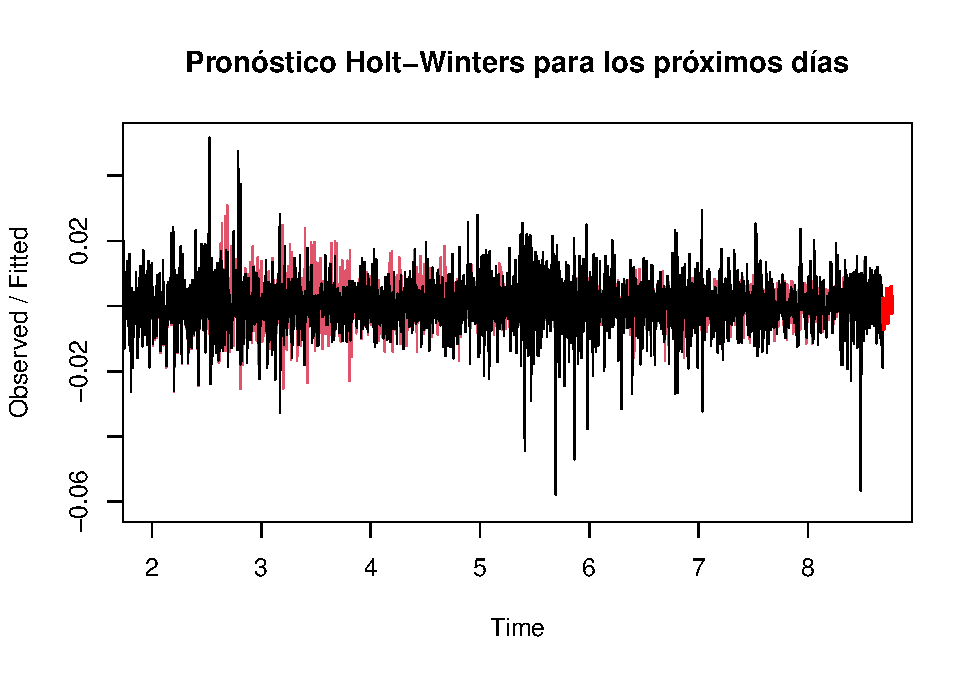
\includegraphics[keepaspectratio]{_main_files/figure-latex/19-1.pdf}}

La línea roja indica el ajuste del modelo sobre la serie temporal. El modelo captura bastante bien la variabilidad

\section{Aplicación de suavizado exponencial simple}\label{aplicaciuxf3n-de-suavizado-exponencial-simple}

\pandocbounded{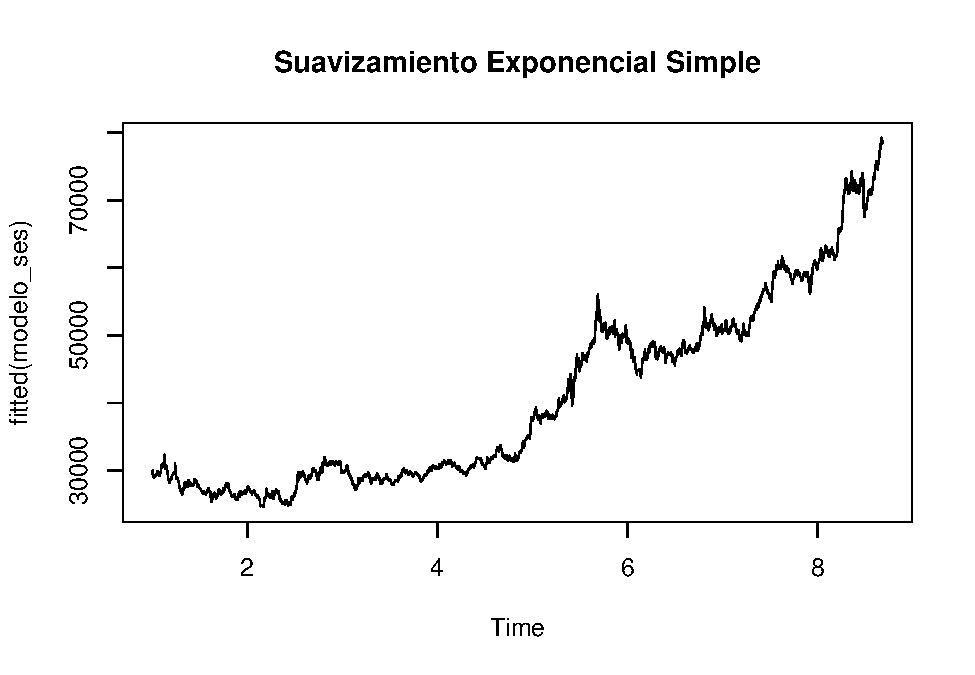
\includegraphics[keepaspectratio]{_main_files/figure-latex/20-1.pdf}}

Este método da más peso a los valores recientes, lo que ayuda a capturar cambios sin reaccionar bruscamente a fluctuaciones
aleatorias.
El modelo Holt-Winters añade tendencia y estacionalidad, mientras que el suavizamiento exponencial simple solo suaviza la
serie.

\section{Comparación de modelos}\label{comparaciuxf3n-de-modelos}

Calcular el error del modelo Holt-Winters

\begin{verbatim}
                    ME        RMSE         MAE MPE MAPE        ACF1 Theil's U
Test set -0.0001721535 0.009329245 0.006690136 NaN  Inf -0.02887819       NaN
\end{verbatim}

Calcular el error del Suavizamiento Exponencial Simple

\begin{verbatim}
               ME     RMSE      MAE        MPE      MAPE         ACF1 Theil's U
Test set 17.38552 353.6919 237.0729 0.03154244 0.5845796 -0.004346762  0.999267
\end{verbatim}

\begin{verbatim}
                            Modelo          MAE         RMSE
1                     Holt-Winters 9.329245e-03 6.690136e-03
2 Suavizamiento Exponencial Simple 3.536919e+02 2.370729e+02
\end{verbatim}

RMSE: 353.69 en modelo SAS, el modelo no ajusta bien la variabilidad de la serie.

MAE: 237.07 También más alto en modelo SAS, indicando errores más grandes en la predicción.

\section{Conclusiones}\label{conclusiones}

\pandocbounded{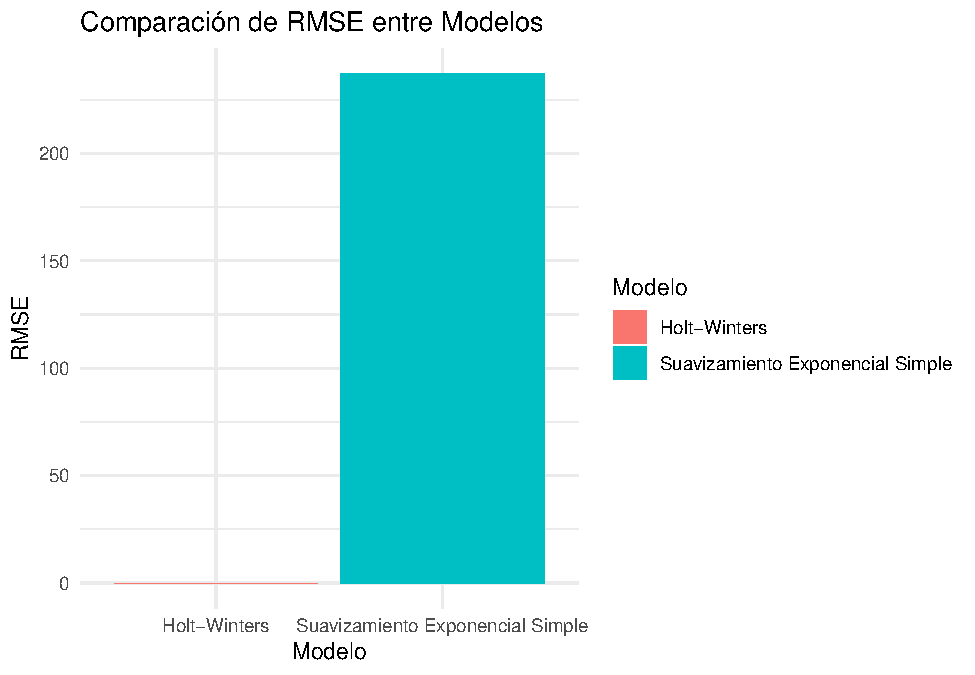
\includegraphics[keepaspectratio]{_main_files/figure-latex/24-1.pdf}}

\begin{itemize}
\tightlist
\item
  Holt-Winters tiene un desempeño mucho mejor en términos de error.
\item
  SES muestra un error muy alto, lo que indica que no captura bien la estructura de la serie. Esto es lógico, ya que el suavizamiento exponencial simple no considera estacionalidad ni tendencia, mientras que Holt-Winters sí lo hace.
\end{itemize}

\chapter{Pronóstico con modelo ARIMA}\label{pronuxf3stico-con-modelo-arima}

\begin{verbatim}
Series: serie_ts 
ARIMA(5,2,0) 

Coefficients:
          ar1      ar2      ar3      ar4      ar5
      -0.8659  -0.6273  -0.4565  -0.3060  -0.1475
s.e.   0.0187   0.0242   0.0255   0.0242   0.0188

sigma^2 = 145160:  log likelihood = -20640.28
AIC=41292.57   AICc=41292.6   BIC=41328.2

Training set error measures:
                     ME     RMSE      MAE          MPE      MAPE       MASE
Training set -0.7881241 380.5229 256.2009 -0.001422517 0.6356454 0.04017145
                    ACF1
Training set -0.01683052
\end{verbatim}

\begin{verbatim}
[1] "AIC: 41292.5656990829"
\end{verbatim}

\begin{verbatim}
[1] "BIC: 41328.1985125718"
\end{verbatim}

\begin{itemize}
\tightlist
\item
  El AIC ayuda a comparar modelos---cuanto más bajo, mejor el ajuste con menos complejidad.
\item
  BIC (Bayesian Information Criterion): Similar a AIC, pero penaliza más la complejidad del modelo. Un BIC menor indica que el modelo es más parsimonioso (no sobreajustado).
\item
  RMSE (Root Mean Squared Error): Mide cuánto se desvían las predicciones de los valores reales. Menor RMSE indica mejor precisión en el ajuste. Para referencia, si el precio del oro oscila en miles, un RMSE de 380 puede ser relativamente aceptable.
\item
  MAE (Mean Absolute Error): Indica el promedio de error absoluto en la predicción
\item
  MAPE (Mean Absolute Percentage Error): Evalúa qué tan bien el modelo predice en términos porcentuales. El modelo tiene buena precisión, con MAPE bajo y errores moderados (RMSE y MAE).
\item
  AIC y BIC sugieren que el modelo es competitivo
\end{itemize}

\pandocbounded{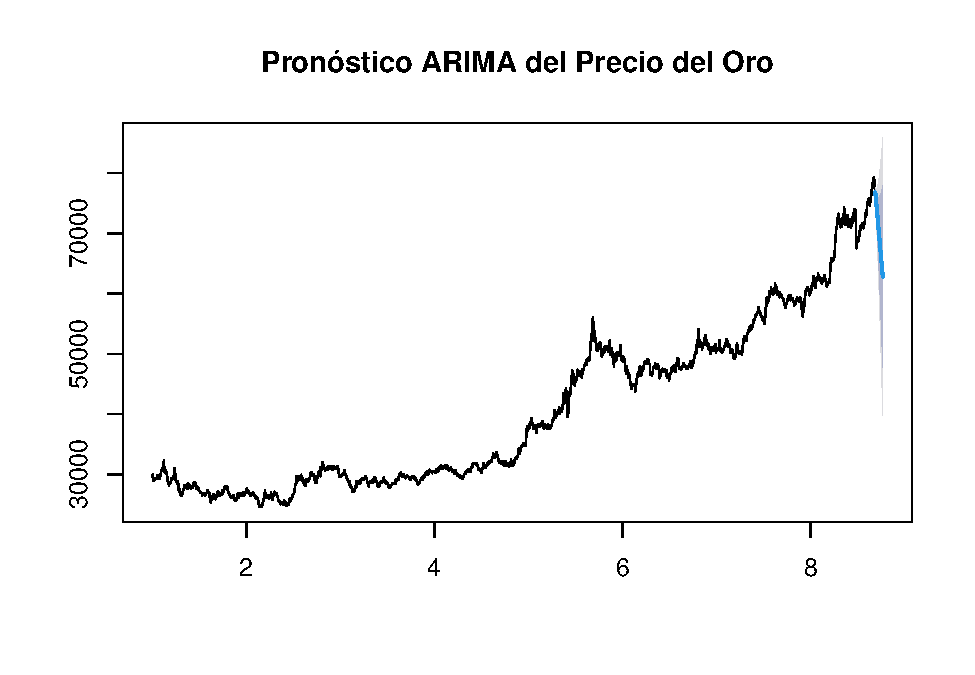
\includegraphics[keepaspectratio]{_main_files/figure-latex/27-1.pdf}}

El modelo predice la evolución del precio del oro basándose en patrones pasados.Dado que ARIMA(5,2,0) usa diferenciación de segundo orden, la predicción busca capturar cambios en la tasa de crecimiento en lugar de los valores absolutos.

\chapter{Algorítmo de Facebook's Prophet}\label{algoruxedtmo-de-facebooks-prophet}

\pandocbounded{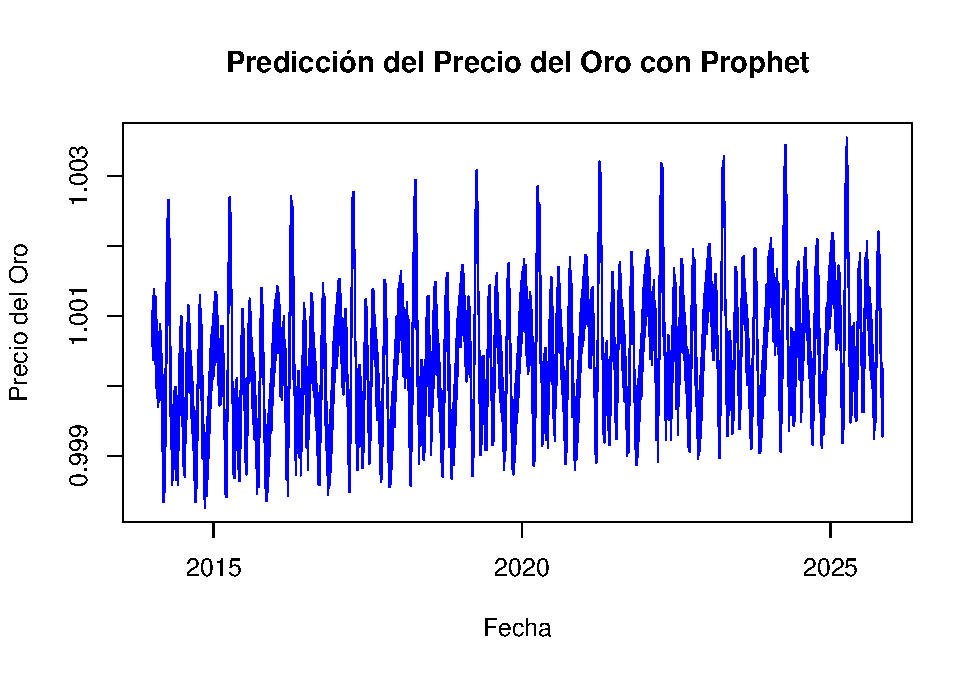
\includegraphics[keepaspectratio]{_main_files/figure-latex/28-1.pdf}}

Recordemos que la serie del precio del oro:

\begin{enumerate}
\def\labelenumi{\arabic{enumi}.}
\tightlist
\item
  Tiene una tendencia clara, con un crecimiento acelerado en ciertos periodos.
\item
  Muestra estacionalidadad, por lo que hay patrones repetitivos a lo largo del tiempo
\item
  Al diferenciarla y aplicar transformación logarítmica, la serie se volvio estacionaria
\end{enumerate}

Una regresión clásica funciona bien cuando hay una relación lineal y estable entre las variables, sin embargo, en casos como estos donde las series temporales tienen
tendencia y estacionalidad, la regresión simple no captura bien los patrones de la serie.

Esta gráfica representa una serie temporal con datos dispersos y una curva de ajuste dada por el algoritmo de Facebook's Prophet (lina azul).

Vemos que la tendencia se mantiene en valores cercanos a cero, lo que significa que después de la transformación logaritmica y diferenciación, los movimientos del precio
del oro son más estacionariarios y predecibles.

En conclusión, usar el método Facebook's prophet es adecuado ya que la serie tiene patrones ciclicos y con este algoritmo se captura mejor la evolución de la serie.

\begin{verbatim}

Call:
lm(formula = y ~ ds, data = df_prophet)

Residuals:
      Min        1Q    Median        3Q       Max 
-0.061581 -0.004095  0.000049  0.004113  0.051570 

Coefficients:
              Estimate Std. Error t value Pr(>|t|)  
(Intercept) -3.785e-03  2.465e-03  -1.535   0.1248  
ds           2.287e-07  1.364e-07   1.677   0.0936 .
---
Signif. codes:  0 '***' 0.001 '**' 0.01 '*' 0.05 '.' 0.1 ' ' 1

Residual standard error: 0.00829 on 2803 degrees of freedom
Multiple R-squared:  0.001003,  Adjusted R-squared:  0.0006462 
F-statistic: 2.813 on 1 and 2803 DF,  p-value: 0.09361
\end{verbatim}

Vemos que el p-valor no es menor que 0.05 para una regresión lineal simple por lo que no es altamente significativa y no capta bien la estructura de la serie.

\chapter{Redes Neuronales}\label{redes-neuronales}

\pandocbounded{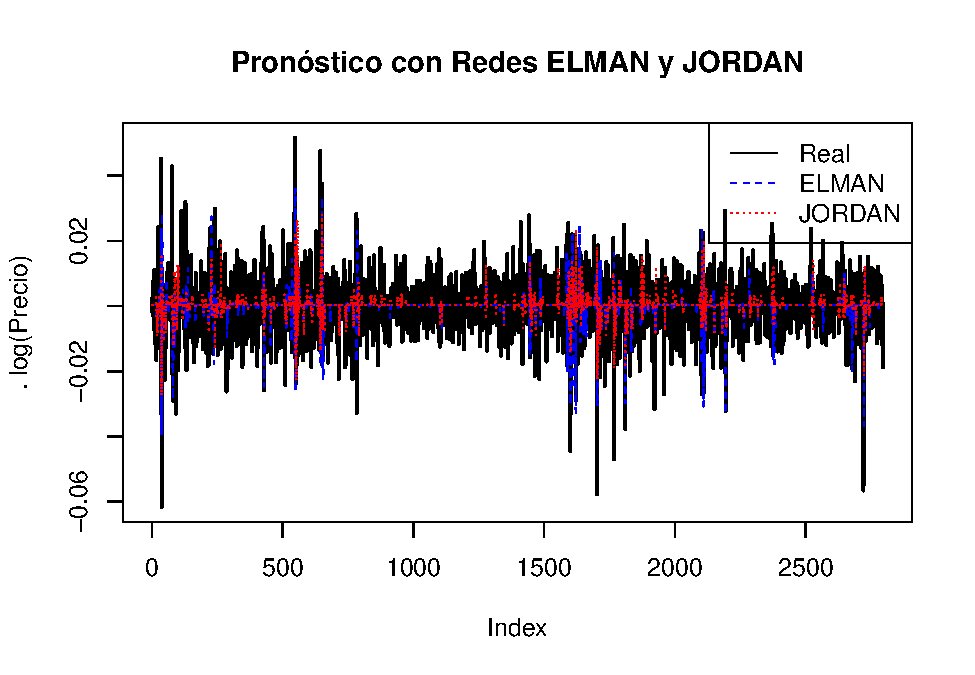
\includegraphics[keepaspectratio]{_main_files/figure-latex/32-1.pdf}}

\begin{verbatim}
  Modelo         MAE        RMSE
1  ELMAN 0.005490801 0.007620683
2 JORDAN 0.005701307 0.007939065
\end{verbatim}

\begin{itemize}
\tightlist
\item
  MAE (Mean Absolute Error): Mide el error promedio absoluto entre las predicciones y los valores reales. ELMAN tiene un MAE ligeramente menor, lo que implica que,
  en promedio, sus predicciones están un poco más cerca de los valores reales.
\item
  RMSE (Root Mean Square Error): Penaliza más los errores grandes. Aquí también ELMAN muestra mejor desempeño con un valor más bajo, lo que sugiere menor
  variabilidad en los errores.
\end{itemize}

Aunque las diferencias son pequeñas, el modelo ELMAN muestra una mejor capacidad de generalización sobre los datos de entrenamiento. Esto sugiere que su arquitectura,
con estados de contexto conectados a las entradas, logra capturar secuencias temporales con mayor precisión que JORDAN, cuyo contexto se retroalimenta desde la salida.

El nivel de error es muy bajo, lo cual habla bien del preprocesamiento y la naturaleza del problema. La serie logarítmica diferenciada se comporta de manera
predecible para este tipo de modelos.

\chapter{Fuentes}\label{fuentes}

\begin{itemize}
\tightlist
\item
  Dataset: \url{https://www.kaggle.com/datasets/nisargchodavadiya/daily-gold-price-20152021-time-series}
\end{itemize}

  \bibliography{book.bib}

\end{document}
